
\begin{figure}[H]
\begin{center}

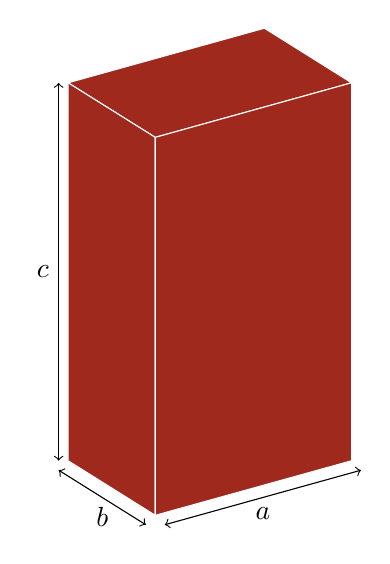
\begin{tikzpicture}[scale = 1.2]

\pgfmathsetmacro{\cubex}{3}
\pgfmathsetmacro{\cubey}{4}
\pgfmathsetmacro{\cubez}{3}
\pgfmathsetmacro{\x}{0}
\pgfmathsetmacro{\y}{0}
\pgfmathsetmacro{\z}{0}

\definecolor{brick}{rgb}{0.62,0.16,0.11}

\draw[white,fill=brick] (\x,\y,\z) -- ++(-\cubex/2,0,-\cubez/2) -- ++(\cubex/2,0,-\cubez/2) -- ++(\cubex/2,0,\cubez/2) -- cycle;
\draw[white,fill=brick] (\x,\y,\z) -- ++(-\cubex/2,0,-\cubez/2) -- ++(0,-\cubey,0) -- ++(\cubex/2,0,\cubez/2) -- cycle;
\draw[white,fill=brick] (\x,\y,\z) -- ++(0,-\cubey,0) -- ++(\cubex/2,0,-\cubez/2) -- ++(0,\cubey,0) -- cycle;

\draw[<->,xshift = .1cm,yshift = -.1cm] (\x,\y -  \cubey,\z) -- ++(\cubex/2,0,-\cubez/2) node[midway,below] {$\mathlarger{a}$};
\draw[<->,xshift = -.1cm,yshift = -.1cm] (\x,\y - \cubey,\z) -- ++(-\cubex/2,0,-\cubez/2) node[midway,below] {$\mathlarger{b}$};
\draw[<->,xshift = -.1cm] (\x - \cubex/2,\y,\z - \cubez/2) -- ++(0.,-\cubey,0.) node[midway,left] {$\mathlarger{c}$};

\end{tikzpicture}
\caption{A rock represented by a regular polyhedron with dimensions $a$, $b$ and $c$.}
\label{fig:rock}
\end{center}
\end{figure}
